
\documentclass[11 pt, titlepage]{article} %Sets the default text size to 11pt and class to article.
%------------------------Dimensions--------------------------------------------
\topmargin=0.0in %length of margin at the top of the page (1 inch added by default)
\oddsidemargin=0.0in %length of margin on sides for odd pages
\evensidemargin=0in %length of margin on sides for even pages
\textwidth=6.5in %How wide you want your text to be
\marginparwidth=0.5in
\headheight=0pt %1in margins at top and bottom (1 inch is added to this value by default)
\headsep=0pt %Increase to increase white space in between headers and the top of the page
\textheight=9.0in %How tall the text body is allowed to be on each page
\setlength\parindent{0pt} % Removes all indentation from paragraphs

%Font
\usepackage[T1]{fontenc}
\usepackage{textcomp}
\usepackage{tgpagella}
\usepackage{lmodern}
\usepackage{fancyvrb}
\usepackage{color}
\usepackage{lipsum}
\usepackage{wrapfig}
\usepackage[utf8]{inputenc}
\usepackage{array, xcolor}
\usepackage{graphicx}
\usepackage{fancyhdr}
\pagestyle{fancy}
\renewcommand{\headrulewidth}{0pt}
\fancyhead{}
\makeatletter
\def\PY@reset{\let\PY@it=\relax \let\PY@bf=\relax%
    \let\PY@ul=\relax \let\PY@tc=\relax%
    \let\PY@bc=\relax \let\PY@ff=\relax}
\def\PY@tok#1{\csname PY@tok@#1\endcsname}
\def\PY@toks#1+{\ifx\relax#1\empty\else%
    \PY@tok{#1}\expandafter\PY@toks\fi}
\def\PY@do#1{\PY@bc{\PY@tc{\PY@ul{%
    \PY@it{\PY@bf{\PY@ff{#1}}}}}}}
\def\PY#1#2{\PY@reset\PY@toks#1+\relax+\PY@do{#2}}

\expandafter\def\csname PY@tok@gd\endcsname{\def\PY@tc##1{\textcolor[rgb]{0.63,0.00,0.00}{##1}}}
\expandafter\def\csname PY@tok@gu\endcsname{\let\PY@bf=\textbf\def\PY@tc##1{\textcolor[rgb]{0.50,0.00,0.50}{##1}}}
\expandafter\def\csname PY@tok@gt\endcsname{\def\PY@tc##1{\textcolor[rgb]{0.00,0.27,0.87}{##1}}}
\expandafter\def\csname PY@tok@gs\endcsname{\let\PY@bf=\textbf}
\expandafter\def\csname PY@tok@gr\endcsname{\def\PY@tc##1{\textcolor[rgb]{1.00,0.00,0.00}{##1}}}
\expandafter\def\csname PY@tok@cm\endcsname{\let\PY@it=\textit\def\PY@tc##1{\textcolor[rgb]{0.25,0.50,0.50}{##1}}}
\expandafter\def\csname PY@tok@vg\endcsname{\def\PY@tc##1{\textcolor[rgb]{0.10,0.09,0.49}{##1}}}
\expandafter\def\csname PY@tok@m\endcsname{\def\PY@tc##1{\textcolor[rgb]{0.40,0.40,0.40}{##1}}}
\expandafter\def\csname PY@tok@mh\endcsname{\def\PY@tc##1{\textcolor[rgb]{0.40,0.40,0.40}{##1}}}
\expandafter\def\csname PY@tok@go\endcsname{\def\PY@tc##1{\textcolor[rgb]{0.53,0.53,0.53}{##1}}}
\expandafter\def\csname PY@tok@ge\endcsname{\let\PY@it=\textit}
\expandafter\def\csname PY@tok@vc\endcsname{\def\PY@tc##1{\textcolor[rgb]{0.10,0.09,0.49}{##1}}}
\expandafter\def\csname PY@tok@il\endcsname{\def\PY@tc##1{\textcolor[rgb]{0.40,0.40,0.40}{##1}}}
\expandafter\def\csname PY@tok@cs\endcsname{\let\PY@it=\textit\def\PY@tc##1{\textcolor[rgb]{0.25,0.50,0.50}{##1}}}
\expandafter\def\csname PY@tok@cp\endcsname{\def\PY@tc##1{\textcolor[rgb]{0.74,0.48,0.00}{##1}}}
\expandafter\def\csname PY@tok@gi\endcsname{\def\PY@tc##1{\textcolor[rgb]{0.00,0.63,0.00}{##1}}}
\expandafter\def\csname PY@tok@gh\endcsname{\let\PY@bf=\textbf\def\PY@tc##1{\textcolor[rgb]{0.00,0.00,0.50}{##1}}}
\expandafter\def\csname PY@tok@ni\endcsname{\let\PY@bf=\textbf\def\PY@tc##1{\textcolor[rgb]{0.60,0.60,0.60}{##1}}}
\expandafter\def\csname PY@tok@nl\endcsname{\def\PY@tc##1{\textcolor[rgb]{0.63,0.63,0.00}{##1}}}
\expandafter\def\csname PY@tok@nn\endcsname{\let\PY@bf=\textbf\def\PY@tc##1{\textcolor[rgb]{0.00,0.00,1.00}{##1}}}
\expandafter\def\csname PY@tok@no\endcsname{\def\PY@tc##1{\textcolor[rgb]{0.53,0.00,0.00}{##1}}}
\expandafter\def\csname PY@tok@na\endcsname{\def\PY@tc##1{\textcolor[rgb]{0.49,0.56,0.16}{##1}}}
\expandafter\def\csname PY@tok@nb\endcsname{\def\PY@tc##1{\textcolor[rgb]{0.00,0.50,0.00}{##1}}}
\expandafter\def\csname PY@tok@nc\endcsname{\let\PY@bf=\textbf\def\PY@tc##1{\textcolor[rgb]{0.00,0.00,1.00}{##1}}}
\expandafter\def\csname PY@tok@nd\endcsname{\def\PY@tc##1{\textcolor[rgb]{0.67,0.13,1.00}{##1}}}
\expandafter\def\csname PY@tok@ne\endcsname{\let\PY@bf=\textbf\def\PY@tc##1{\textcolor[rgb]{0.82,0.25,0.23}{##1}}}
\expandafter\def\csname PY@tok@nf\endcsname{\def\PY@tc##1{\textcolor[rgb]{0.00,0.00,1.00}{##1}}}
\expandafter\def\csname PY@tok@si\endcsname{\let\PY@bf=\textbf\def\PY@tc##1{\textcolor[rgb]{0.73,0.40,0.53}{##1}}}
\expandafter\def\csname PY@tok@s2\endcsname{\def\PY@tc##1{\textcolor[rgb]{0.73,0.13,0.13}{##1}}}
\expandafter\def\csname PY@tok@vi\endcsname{\def\PY@tc##1{\textcolor[rgb]{0.10,0.09,0.49}{##1}}}
\expandafter\def\csname PY@tok@nt\endcsname{\let\PY@bf=\textbf\def\PY@tc##1{\textcolor[rgb]{0.00,0.50,0.00}{##1}}}
\expandafter\def\csname PY@tok@nv\endcsname{\def\PY@tc##1{\textcolor[rgb]{0.10,0.09,0.49}{##1}}}
\expandafter\def\csname PY@tok@s1\endcsname{\def\PY@tc##1{\textcolor[rgb]{0.73,0.13,0.13}{##1}}}
\expandafter\def\csname PY@tok@sh\endcsname{\def\PY@tc##1{\textcolor[rgb]{0.73,0.13,0.13}{##1}}}
\expandafter\def\csname PY@tok@sc\endcsname{\def\PY@tc##1{\textcolor[rgb]{0.73,0.13,0.13}{##1}}}
\expandafter\def\csname PY@tok@sx\endcsname{\def\PY@tc##1{\textcolor[rgb]{0.00,0.50,0.00}{##1}}}
\expandafter\def\csname PY@tok@bp\endcsname{\def\PY@tc##1{\textcolor[rgb]{0.00,0.50,0.00}{##1}}}
\expandafter\def\csname PY@tok@c1\endcsname{\let\PY@it=\textit\def\PY@tc##1{\textcolor[rgb]{0.25,0.50,0.50}{##1}}}
\expandafter\def\csname PY@tok@kc\endcsname{\let\PY@bf=\textbf\def\PY@tc##1{\textcolor[rgb]{0.00,0.50,0.00}{##1}}}
\expandafter\def\csname PY@tok@c\endcsname{\let\PY@it=\textit\def\PY@tc##1{\textcolor[rgb]{0.25,0.50,0.50}{##1}}}
\expandafter\def\csname PY@tok@mf\endcsname{\def\PY@tc##1{\textcolor[rgb]{0.40,0.40,0.40}{##1}}}
\expandafter\def\csname PY@tok@err\endcsname{\def\PY@bc##1{\setlength{\fboxsep}{0pt}\fcolorbox[rgb]{1.00,0.00,0.00}{1,1,1}{\strut ##1}}}
\expandafter\def\csname PY@tok@kd\endcsname{\let\PY@bf=\textbf\def\PY@tc##1{\textcolor[rgb]{0.00,0.50,0.00}{##1}}}
\expandafter\def\csname PY@tok@ss\endcsname{\def\PY@tc##1{\textcolor[rgb]{0.10,0.09,0.49}{##1}}}
\expandafter\def\csname PY@tok@sr\endcsname{\def\PY@tc##1{\textcolor[rgb]{0.73,0.40,0.53}{##1}}}
\expandafter\def\csname PY@tok@mo\endcsname{\def\PY@tc##1{\textcolor[rgb]{0.40,0.40,0.40}{##1}}}
\expandafter\def\csname PY@tok@kn\endcsname{\let\PY@bf=\textbf\def\PY@tc##1{\textcolor[rgb]{0.00,0.50,0.00}{##1}}}
\expandafter\def\csname PY@tok@mi\endcsname{\def\PY@tc##1{\textcolor[rgb]{0.40,0.40,0.40}{##1}}}
\expandafter\def\csname PY@tok@gp\endcsname{\let\PY@bf=\textbf\def\PY@tc##1{\textcolor[rgb]{0.00,0.00,0.50}{##1}}}
\expandafter\def\csname PY@tok@o\endcsname{\def\PY@tc##1{\textcolor[rgb]{0.40,0.40,0.40}{##1}}}
\expandafter\def\csname PY@tok@kr\endcsname{\let\PY@bf=\textbf\def\PY@tc##1{\textcolor[rgb]{0.00,0.50,0.00}{##1}}}
\expandafter\def\csname PY@tok@s\endcsname{\def\PY@tc##1{\textcolor[rgb]{0.73,0.13,0.13}{##1}}}
\expandafter\def\csname PY@tok@kp\endcsname{\def\PY@tc##1{\textcolor[rgb]{0.00,0.50,0.00}{##1}}}
\expandafter\def\csname PY@tok@w\endcsname{\def\PY@tc##1{\textcolor[rgb]{0.73,0.73,0.73}{##1}}}
\expandafter\def\csname PY@tok@kt\endcsname{\def\PY@tc##1{\textcolor[rgb]{0.69,0.00,0.25}{##1}}}
\expandafter\def\csname PY@tok@ow\endcsname{\let\PY@bf=\textbf\def\PY@tc##1{\textcolor[rgb]{0.67,0.13,1.00}{##1}}}
\expandafter\def\csname PY@tok@sb\endcsname{\def\PY@tc##1{\textcolor[rgb]{0.73,0.13,0.13}{##1}}}
\expandafter\def\csname PY@tok@k\endcsname{\let\PY@bf=\textbf\def\PY@tc##1{\textcolor[rgb]{0.00,0.50,0.00}{##1}}}
\expandafter\def\csname PY@tok@se\endcsname{\let\PY@bf=\textbf\def\PY@tc##1{\textcolor[rgb]{0.73,0.40,0.13}{##1}}}
\expandafter\def\csname PY@tok@sd\endcsname{\let\PY@it=\textit\def\PY@tc##1{\textcolor[rgb]{0.73,0.13,0.13}{##1}}}

\def\PYZbs{\char`\\}
\def\PYZus{\char`\_}
\def\PYZob{\char`\{}
\def\PYZcb{\char`\}}
\def\PYZca{\char`\^}
\def\PYZam{\char`\&}
\def\PYZlt{\char`\<}
\def\PYZgt{\char`\>}
\def\PYZsh{\char`\#}
\def\PYZpc{\char`\%}
\def\PYZdl{\char`\$}
\def\PYZhy{\char`\-}
\def\PYZsq{\char`\'}
\def\PYZdq{\char`\"}
\def\PYZti{\char`\~}
% for compatibility with earlier versions
\def\PYZat{@}
\def\PYZlb{[}
\def\PYZrb{]}
\makeatother

% pygmentize -f latex function.java > output.tex

\usepackage[hidelinks]{hyperref}
\usepackage{framed}

\definecolor{dark-red}{rgb}{0.4,0.15,0.15}
\definecolor{dark-blue}{rgb}{0.15,0.15,0.4}
\definecolor{medium-blue}{rgb}{0,0,0.5}
\hypersetup{
    colorlinks, linkcolor={dark-red},
    citecolor={dark-blue}, urlcolor={medium-blue}
}


\begin{document}


\title{Kommunikation och Användargränssnitt - Android utveckling}
\author{Andreas Valter \and Fredrik Lindner \and  \and Karl-Johan Krantz \and Jonas Strandstedt \and Jonas Zeitler }
\maketitle

\section{Syfte}
Denna laboration är en introduktion till Android programmering för att ni ska ha möjlighet att göra en mobilapp som projekt. 
Ni kommer även att få en introduktion till hur man använder enklaste möjliga databas tillsammans med Android, det möjliggör applikationer med mer avancerade data.
\section{Inledning}
Uppgiften är att göra en “Att göra lista” med möjlighet att lägga till och ta bort uppgifter.
\section{Installation}
För att installera Android SDK gå in på \href{http://developer.android.com/sdk/index.html}{http://developer.android.com/sdk/index.html} och välj “Download the SDK, ADT Bundle for Windows”. Utvecklingsmiljön är en färdigkonfigurerat version av Eclipse och finns till Windows, Linux och Mac.\\

Packa upp zip-filen till D: och öppna Eclipse från “adt-bundle-win-x86\_64-yyyymmdd/eclipse/eclipse.exe”. 
Första gången du öppnar Eclipse kommer den fråga efter var du ska placera dess workspaces. 
Vi föreslår att du väljer en mapp som finns på “private\_stuff”, vi kommer skapa en mapp och använda “H:/Workspace”.

\subsection{Skapa en Android Emulator}
För att kunna köra en Android applikation behövs en Android enhet. 
Eftersom vi inte utgår från att alla har en Android telefon/platta föreslår vi att installera en Android emulator. 
“Window -> Android Virtual Device Manager”, välj sedan “New...”.

AVD Name: MyDevice\\
Device:  Nexus 7\\
Target:  Android 4.3 - API Level 18\\
Emulating Options:  Use host GPU\\
Lämna resten som default.\\

\subsection{Skapa Projektet}
Nu har du startat Eclipse samt skapat en enhet. 
Nu är det dags för det roliga, koda!\\

Välj “File -> New -> Android Application Project”\\ 
Application Name:  MyToDoList\\
Minimum Required SDK:  API 11: Android 3.0 (Honeycomb)\\
Fortsätt genom att använda default inställningarna på resten av valen och avsluta med “Finish”. 
Nu kan ditt fönster fortfarande ha en välkomstmeny till Android SDK. 
Avsluta den med krysset som är uppe i vänstra hörnet i den inre ramen.

Kör din Androidapplikation genom att trycka på “Play” knappen i menyn eller Ctrl+F11. 
Notera att Androidemulatorn tar några minuter att starta första gången. 
Stäng inte av emulatorn med krysset mellan körningar för då tar det lång tid att starta varje gång.

\section{Todo Applikation}
Vi kommer inte att gå in på djupet i hur Android fungerar. 
För er som arbetat med iOS tidigare kommer att märka att det skiljer sig en hel del och att hur vyer hanteras är annorlunda. 
Fokus på labben kommer vara att arbeta i Java och nödvändiga Androidspecifika komponenter kommer att ges.
\begin{figure}[ht!]
\centering
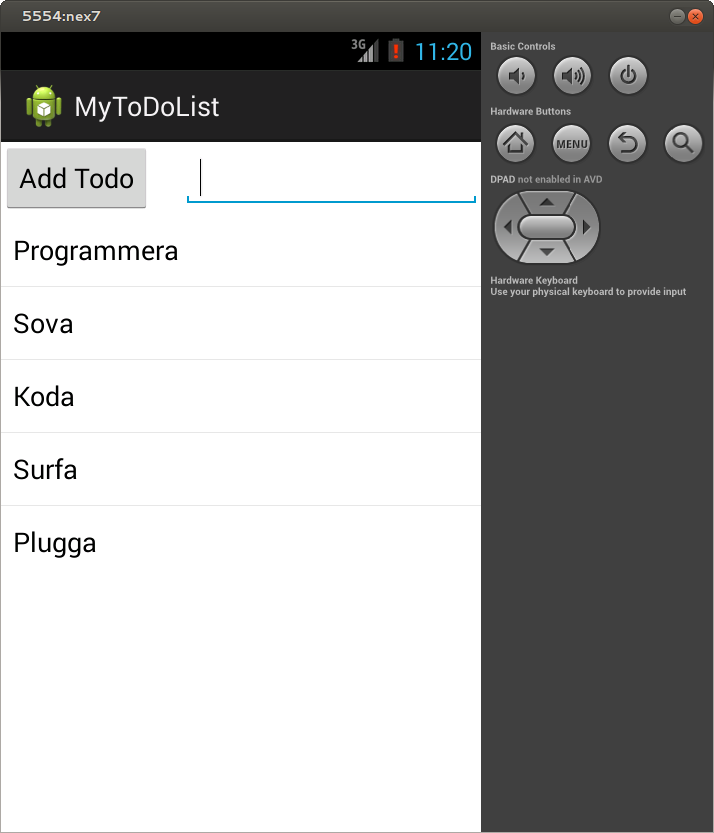
\includegraphics[width=90mm]{images/app.png}
\caption{Exempel på hur en färdig ToDo-app kan se ut.}
\label{overflow}
\end{figure}
\subsection{Debug prints}
För den som är van att arbeta med textbaserade program är det vanligt att göra “debug prints” för att kontrollera att värden i variabler är korrekt samt se att funktioner blivit anropade etc.

Öppna först Android logcat genom “\textit{Window -> Show View -> Other..}”, Välj “\textit{Android -> LogCat}”.\\
Varje logmeddelande görs med att ge ett meddelande en tagg som identifierar vad den hör till. 
Exempelvis “databas”, “info” eller debug”. 
Vi kommer använda “TodoLog”. 
När logcat är öppnad behöver vi skapa ett filter, för Android kommer att spotta ut väldigt mycket meddelanden och vi är just nu enbart intresserade av “TodoLog”.\\ 
Tryck på det gröna plusset.\\

Välj ett namn för ditt filter och välj “by Log Tag” där ni fyller i det namn på taggen ni vill filtrera efter.\\ \\
Testa att det fungerar genom att logga i funktionen onCreate.
\begin{Verbatim}[commandchars=\\\{\}]
\PY{n}{Log}\PY{o}{.}\PY{n+na}{d}\PY{o}{(}\PY{l+s}{\PYZdq{}TodoLog\PYZdq{}}\PY{o}{,} \PY{l+s}{\PYZdq{}Programmet startat\PYZdq{}}\PY{o}{)}\PY{o}{;}
\end{Verbatim}


\subsection{Visa en lista}
För att kunna skapa en lista med saker att göra är det lämpligt att först skapa den grafiska layouten för listan. Det grafiska gränssnittet ligger i filen “\textit{res -> layout -> activity\_main.xml}”.\\
I Eclipse så kan du enkelt navigera till filen i “Package Explorer”. Dubbelklicka för att öppna den.\\

Nu bör du få upp hur det grafiska gränssnittet ser ut i en mobiltelefon/surfplatta. Här kan du direkt redigera gränssnittet genom att dra in olika element ifrån “Palette” eller redigera XML-koden genom att byta ifrån “Graphical layout” till “activity\_main.xml” i nedre delen av fönstret. Du behöver inte välja antingen eller, men det är bra att ha koll på båda.\\

Textfältet “Hello World!” kan du bara ta bort genom att antingen markera det direkt eller markera det i listan “Outline” till höger, och trycka på delete.\\ 

Skapa en lista genom att dra in elementet “\textit{Composite -> ListView}”. För att våran aktivitet i appen ska kunna nå listan så måste den få ett lite annorlunda “id” än vad den har nu. I “\textit{Properties}” finns det ett fält som heter “Id”. Ändra innehållet i den till “\textit{@android:id/list}”. Detta är lite speciellt när det kommer till just en lista och vi kommer senare att behandla id på ett lite mer konventionellt sätt när det kommer till knappar och textfält.\\

Nu kan du återgå till koden i filen MainActivity.java, som innehåller källkoden för huvudaktiviteten i din app.
Då vi har valt att skapa en lista i vår Activity, så gör vi bäst i att ärva från ListActivity istället för Activity i vår klass.
Ändra så att MainActivity ärver ifrån ListActivity istället för Activity. \\

Eclipse vet inte automatiskt vad en ListActivity är och markerar detta som ett fel i koden. Importera klassen genom att klicka på det rödmarkerade ListActivity och välj “Import ‘ListActivity’ (android.app)”. Eclipse har även ett snabbkommando (ctrl+shift+o) för att hantera vad som behöver importeras.\\

För att göra en enkel lista att testa ditt grafiska gränsnitt med, så behövs det lite data att visa.
Ge din klass en privat datamedlem som är en String ArrayList och döp den till testData. ArrayList är i syntaxen ganska lik Vector, som du nog är bekant med sedan tidigare.
Deklarera även en privat datamedlem av klassen ArrayAdapter som tar typen String och döp en till adapter.\\


I metoden onCreate, som anropas direkt efter appen har startats, kan du instansiera din String ArrayList med lite testdata. Här gör du som du vill, ett sätt är bara loopa igenom arrayen och lägga in en siffra eller textsnutt för varje index.\\

Nu måste vi koppla denna data till vårt grafiska gränssnitt. Detta är inte helt intuitivt till en början, så ni får lite hjälp med det:
\begin{Verbatim}[commandchars=\\\{\}]
\PY{n}{adapter} \PY{o}{=} \PY{k}{new} \PY{n}{ArrayAdapter}\PY{o}{\PYZlt{}}\PY{n}{String}\PY{o}{\PYZgt{}}\PY{o}{(}\PY{k}{this}\PY{o}{,} \PY{n}{android}\PY{o}{.}\PY{n+na}{R}\PY{o}{.}\PY{n+na}{layout}\PY{o}{.}\PY{n+na}{simple\PYZus{}list\PYZus{}item\PYZus{}1} \PY{o}{,} \PY{n}{testData}\PY{o}{)}\PY{o}{;}
\PY{n}{setListAdapter}\PY{o}{(}\PY{n}{adapter}\PY{o}{)}\PY{o}{;}
\end{Verbatim}

Det som sker här är att vi skapar en s.k ArrayAdapter som kopplar ihop datan som är lagrad i testData med det grafiska gränsnittet. Vi anger vilken datatyp det är (String) och var datan är lagrad (testData). Tillslut tilldelar vi adaptern till aktiviteten via setListAdapter.\\

Om allt har gått rätt till så bör nu appen kunna startas genom att trycka på Run. Appen bör startas i Android emulatorn. En lista, som förvisso är rätt tråkig och statisk, bör nu visas!\\ \\


\fbox{
  \parbox{\textwidth}{
	\textbf{Uppgift:} Gör en lista i det grafiska gränssnittet.
	Skapa en ArrayList av typen String, initialisera den med lite data
	och koppla ihop det med en ArrayAdapter, också av typen String.
	}
}
\subsection{Interagera (click event) med en lista}
Nu är det dags att få igång interaktionen med listan. Eftersom vår \textit{MainActivity} ärver av \textit{ListActivity}, så är det ganska enkelt att komma igång med.\\

För att skapa en event listener som lyssnar på interaktioner med listan ska vi överlagra metoden \textit{onListItemClick} från \textit{ListActivity}. Här kan vi använda Eclipse för att generera en metodsignatur. Ställ markören någonstans i klassen \textit{MainActivity} (men inte i någon metod), börja skriva \textit{“onListItemClick”} och tryck ctrl+space. Eclipse föreslår då att infoga en överlagrad variant av \textit{onListItemClick} från \textit{ListActivity} med alla funktionsparametrar som behövs.\\

OBS! Notera att du behöver ändra så att de två sista argumenten är konstanta, dvs \textit{final int} respektive \textit{final long}. Detta behövs senare för att ha tillgång till dem i en lyssnare.\\

Inne i metoden kan vi nu bestämma vad som ska hända när en användare klickar på en rad i listan. Enklast just nu är förstås att bara logga till LogCat.\\

När du nu kör din app igen, så bör LogCat visa din text när man trycker på en post i listan.\\ \\
\fbox{
  \parbox{\textwidth}{
	\textbf{Uppgift:} Implentera onListItemClick och skriv ut någon text genom LogCat för att se att interaktionen med listan funkar korrekt. 
	}
}
\subsection{Visa en popup}
Nu när vi vet att det funkar att klicka på en post i listan, så kanske det kan vara roligare att få upp ett meddelande i appen istället för LogCat.

Tidigare så såg vi att man enkelt kunde utforma sitt grafiska gränssnitt med den grafiska editorn. Det kan man använda för mer eller mindre allt grafiskt arbete, men när det kommer till enklare saker som tex dialogrutor kan det vara lämpligt att skriva de direkt i koden.

För att göra detta använder vi oss av en \textit{Builder} till komponenten \textit{AlertDialog}. \textit{AlertDialog} visar en popup dialog anpassad för saker som att bekräfta en återgärd eller visa information om en post.

\begin{Verbatim}[commandchars=\\\{\}]
\PY{n}{AlertDialog}\PY{o}{.}\PY{n+na}{Builder} \PY{n}{builder} \PY{o}{=} \PY{k}{new} \PY{n}{AlertDialog}\PY{o}{.}\PY{n+na}{Builder}\PY{o}{(}\PY{k}{this}\PY{o}{)}\PY{o}{;}
\end{Verbatim}

Vi kan nu lägga till saker i våran builder. Anropa metoden setMessage med en sträng som argument för att sätta ett textmeddelande som dyker upp när man trycket på en post.

Vi har ännu inte skapat våran \textit{AlertDialog}, men det gör vi nu genom att anropa 
\begin{Verbatim}[commandchars=\\\{\}]
\PY{n}{AlertDialog} \PY{n}{dialog} \PY{o}{=} \PY{n}{builder}\PY{o}{.}\PY{n+na}{create}\PY{o}{(}\PY{o}{)}\PY{o}{;}
\end{Verbatim}

Sedan kan vi visa dialog genom dialog.show();
Kör appen och se hur du nu får en popup ruta med texten när du klickar på en post!\\ \\
\fbox{
  \parbox{\textwidth}{
	\textbf{Uppgift:} Använd dig av \textit{AlertDialog} och dess tillhörande \textit{Builder} för att skapa en dialogruta som visas när man trycker på en post i listan.
	}
}

\section{Ta bort poster}
Låt oss nu försöka lägga till funktionalitet för att kunna ta bort en post ifrån listan. 
Med metoderna setPositiveButton och setNegativeButton på builder-objektet kan man enkelt få upp två knappar som man kan styra hur man vill. Båda två metoderna tar två argument; en sträng för texten på knappen och en OnClickListener.
Här kan du antingen anropa en lyssnare som du skapat någon annanstans, eller helt enkelt skapa den direkt i metodanropet genom 
\begin{Verbatim}[commandchars=\\\{\}]
\PY{k}{new} \PY{n}{DialogInterface}\PY{o}{.}\PY{n+na}{OnClickListener}\PY{o}{(}\PY{o}{)} \PY{o}{\PYZob{}} \PY{o}{\PYZcb{}}
\end{Verbatim}


Inuti denna lyssnare så måste metoden \textit{onClick(DialogInterface, int)} finnas. Det är alltså här inne som funktionaliteten för att kunna ta bort en post ifrån listan skall implementeras.\\

För att ta bort en post ifrån listan så behöver du anropa metoden \textit{remove} på medlemmen adapter. remove tar i det här fallet ett objekt av typen String som argument, då ArrayAdapter:n har blivit deklarerad för att hantera just String. Här vill du nu plocka bort den aktuella posten i listan genom att hitta den i testData.
I argumenten för \textit{onListItemClick} så finns den aktuella postens index i konstanten \textit{id}.\\  
Om du gjort rätt så kommer posten tas bort från både testData och adapter, vilket kommer resultera i att listan i det grafiska gränssnittet uppdateras korrekt.\\

Knappen för “Ok” behöver inte göra någonting, så hela onClick-metoden kan bara vara tom.\\

\begin{figure}[ht!]
\centering
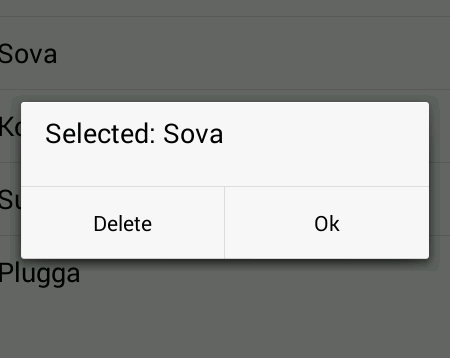
\includegraphics[width=90mm]{images/popup.png}
\caption{AlertDialog med möjlighet att ta bort den aktuella posten i listan.}
\label{overflow}
\end{figure} \\

\fbox{
  \parbox{\textwidth}{
	\textbf{Uppgift:} Skapa två knappar i dialogrutan, en som bara är “Ok” och inte gör något mer än att stänga rutan, och en “Delete” som tar bort den aktuella posten från listan.
	}
}

\subsection{Knappar och textfält}
Det hade naturligtvis varit trevligt med möjligheten att lägga till nya poster i listan. För att göra det behöver vi en knapp för att lägga till, och ett textfält för att skriva in namnet.\\

Gå tillbaka till ditt grafiska gränssnitt (\textit{activity\_main.xml}). För att göra en smidig layout så behöver vi först ändra lite. I \textit{Outline}, högerklicka på \textit{RelativeLayout} och välj \textit{Change layout...}. Välj sedan \textit{LinearLayout(vertical)}. Inuti denna \textit{LinearLayout} så finns du din lista. Skapa ytterligare en \textit{LinearLayout}, men en som är horizontal. Lägg den inuti den första \textit{LinearLayout(vertical)}. Titta i \textit{Outline} så att din nya \textit{LinearLayout(horizontal)} ligger inuti den andra \textit{LinearLayout}, och ovanför listan.\\

Lägg nu till en knapp(\textit{Form Widgets -> Button}) och ett textfält (\textit{Text Fields -> Plain Text}) så de hamnar i din \textit{LinearLayout(horizontal)}. Ge dem ett lämpligt \textit{id} i \textit{Properties}, tex "add" för knappen och "name" för textfältet. Kom ihåg att det måste vara på formen \textit{@+id/ditt-namn-här}.\\

\begin{figure}[ht!]
\centering
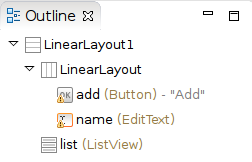
\includegraphics[width=90mm]{images/outline.png}
\caption{Outline med alla elementen inlagda.}
\label{overflow}
\end{figure} \\

Om du testkör din app nu, så bör du se både knappen och textfältet som det ser ut när du designar ditt grafiska gränssnitt, men de gör inget än så låt oss fixa det. \\

För att kunna interagera med knappen så behöver vi lägga till lyssnare. Detta gör vi i onCreate metoden.
Skapa först knappen genom \begin{Verbatim}[commandchars=\\\{\}]
\PY{n}{Button} \PY{n}{button} \PY{o}{=} \PY{o}{(}\PY{n}{Button}\PY{o}{)}\PY{n}{findViewById}\PY{o}{(}\PY{n}{R}\PY{o}{.}\PY{n+na}{id}\PY{o}{.}\PY{n+na}{add}\PY{o}{)}\PY{o}{;}
\end{Verbatim}


Nu kan vi anropa metoden \textit{setOnClickListener} på \textit{button}. Som tidigare kan vi skapa en lyssnare direkt i metodanropet
\begin{Verbatim}[commandchars=\\\{\}]
\PY{k}{new} \PY{n}{View}\PY{o}{.}\PY{n+na}{OnClickListener}\PY{o}{(}\PY{o}{)} \PY{o}{\PYZob{}} \PY{o}{\PYZcb{}}
\end{Verbatim}


Som tidigare behövs en överladdad metod \textit{onClick(View)} i lyssnaren (av typen \textit{public void}). Innan vi kan definera vad knappen ska göra när användaren trycker på den, så måste vi identifiera att användaren har tryckt just på våran knapp.
I \textit{onClick} så har vi fått med en View som har den tillhörande metoden \textit{getId()} för att hämta id på det elementet som har aktivierats. Se till så att det överensstämmer med id på våran knapp genom att jämföra med \textit{R.id.add} (dvs, om knappen är döpt till "add").\\

Nu måste vi hämta ut informationen som är inskrivet i textfältet! På samma sätt som knappen skapades ovan så kan vi skapa ett textfält, som är av typen \textit{EditText} istället för \textit{Button}.
Metoden \textit{getText()} hämtar ut text från ett textfält, dock är det inte av typen String. Fixa det!\\

Sen är det bara att lägga in texten i form av en String i \textit{adapter}. Det är väldigt likt det vi gjorde tidigare när vi tog bort elementet ur \textit{adapter}...\\ \\
\fbox{
  \parbox{\textwidth}{
	\textbf{Uppgift:} Skapa en knapp och ett textfält. När man trycker på knappen skall texten som är i textfältet läggas till i listan.
	}
}
\section{Databaskoppling}
Hittills har vi endast lagrat data i en ArrayList. Den tas naturligtvis bort så fort programmet stängs ned. Ett smidigare sätt att lagra data för en ToDo-lista är att lagra allt i en liten SQL databas. All kod för att skapa en databas och lagra en egen klass i den är redan skriven, och finns i filerna \textit{MySQLiteHelper.java}, \textit{TodosDataSource.java} och \textit{Todo.java}.\\

Här är det ett bra ställe att klippa navelsträngen, nedan ges bara de metoderna som kan vara användbara för att få det att funka med databasen. Allt är redan färdigt i de filerna som skickas med så inget behöver ändras där, men kolla i dom för att förstå hur det hänger ihop. Försök komma så långt ni kan!\\ \\

Datamedlemmar: ArrayList av typen Todo, ArrayAdapter av typen Todo, TodosDataSource \\
TodosDataSource metoder: open(), getAllTodos(), createTodo(), deleteTodo() \\

\fbox{
  \parbox{\textwidth}{
  	\textbf{Uppgift:} Skapa en ToDo-list app med koppling till en databas.
  }
}
\\ \\

Lycka till!



\end{document}
